\usepackage[authoryear,round]{natbib}
\usepackage{multirow}
\usetikzlibrary{decorations.pathmorphing}

\newcommand{\sheetnum}{%
	01
}
%\setcounter{section}{\sheetnum-3}
\newcommand{\tutorialtitle}{%
    Principal Component Analysis
}
\newcommand{\tutorialtitleshort}{%
	PCA
}
% for slides
\subtitle{\sheetnum \tutorialtitle}

%\maxdeadcycles=1000 % Workaround for ! Output loop---100 consecutive dead cycles because of too many figures

% The following use of algroithms does not work well with the notes:
%
%
%
%
% instead use the following for your algorithms:
%
%\begin{figure}[!t]
%\removelatexerror
%\begin{algorithm}[H]
    % your algo here
    %\label{alg:algolabel}
    %\caption{algocaption}
%\end{algorithm}
%\end{figure}
%\begin{algorithm}
% Below is the definition for the command \removelatexerror:
\makeatletter
\newcommand{\removelatexerror}{\let\@latex@error\@gobble}
\makeatother

\begin{document} %%%%%%%%%%%%%%%%%%%%%%%%%%%%%%%%%%%%%%%%%%%%%%%%%%%%%%%

\sheet{\sheetnum}{\tutorialtitleshort}

\ttopic{\tutorialtitle}

\columnratio{0.2,0.8}\textbf{}
\begin{paracol}{2}
%\setlength{\columnseprule}{0.1pt}
%\setlength{\columnsep}{5em}

\begin{rightcolumn}

% notes version will ignore it
\begin{frame}
\titlepage
\end{frame}

\begin{frame}
\tableofcontents
\end{frame}

\newpage

\mode<all>
\section{The setting}

\begin{frame}\frametitle{\secname}
    
\underline{Data:}

observations: $\big\{ \vec{x}^{(\alpha)} \big\}, \alpha = 1, \ldots, p; \quad \vec{x} \in \R^N$

$$
\vec x = \rmat{
x_1\\
x_2\\
\vdots\;\,\\
x_N
}
$$

Our entire dataset:
\[
\vec X = 
\left(
\begin{array}{cccc}
\Big| & \Big| & &\Big| \\[3mm]
\vec x^{(1)} & \vec x^{(2)} & \cdots &\vec x^{(p)}\\[2mm]
\Big| & \Big| & &\Big|
\end{array}
\right) \in \R^{N \times p}
\]

\end{frame}

\section{Dimensionality Reduction}

\begin{frame}\frametitle{\secname}
We want to reduce the number of elements in $\vec x \in \R^N$
while retaining as most of the intrinsic information content.

\question{For what purpose?}

\question{What is the difference between dimensionality reduction and compression, if any?}

\end{frame}

%\newpage
\subsection{Simple truncation}




\begin{frame}\frametitle{\subsecname}

\begin{center}
\begin{minipage}{0.3\textwidth}

	%\begin{table}[]
	%\centering
	\resizebox{\textwidth}{!}{%
	\begin{tabular}{c|cccc}
			  & \multicolumn{1}{c}{$\vec x^{(1)}$} & \multicolumn{1}{c}{$\vec x^{(2)}$} & \multicolumn{1}{c}{\ldots} & $\vec x^{(p)}$ \\ \hline%\cline{1-3} \cline{5-5} 
	$x_1$     & -0.2                           & 0.1                            &                       & 0.2       \\ \cline{1-1}
	$x_2$     & 0.1                            & 3.1                            &                       & -1.0      \\ \cline{1-1}
	$x_3$     & 2.5                            & 7.2                            &                       & -0.8      \\ %\cline{1-1}
	  \vdots        &            \vdots                    &     \vdots                          & \begin{tabular}[c]{@{}c@{}}\ldots\vspace{2.5mm}\end{tabular} &      \vdots     \\ %\cline{1-1}
	$x_{N-2}$ & -7.1                           & -3.5                           &                       & 7.0       \\ \cline{1-1}
	$x_{N-1}$ & -10.3                          & -0.3                           &                       & 4.5       \\ \cline{1-1}
	$x_N$     & 4.0                            & 1.3                            &                       & 6.6       \\ \hline
	\end{tabular}%
	}
	%\end{table}
\end{minipage}
\begin{minipage}{0.33\textwidth}
	\begin{center}
		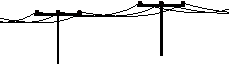
\includegraphics[width=0.99\textwidth]{img/telephone_masts_depth}%
	\end{center}
\end{minipage}
\begin{minipage}{0.3\textwidth}

	\resizebox{\textwidth}{!}{%
	\begin{tabular}{c|cccc}
			  & \multicolumn{1}{c}{$\vec x^{(1)}$} & \multicolumn{1}{c}{$\vec x^{(2)}$} & \multicolumn{1}{c}{\ldots} & $\vec x^{(p)}$ \\ \hline%\cline{1-3} \cline{5-5} 
	$x_1$     & -0.2                           & 0.1                            &                       & 0.2       \\ \cline{1-1}
	$x_2$     & 0.1                            & 3.1                            &                       & -1.0      \\ \cline{1-1}
	$x_3$     & 2.5                            & 7.2                            &                       & -0.8      \\ %\cline{1-1}
	  \vdots        &            \vdots                    &     \vdots                          & \begin{tabular}[c]{@{}c@{}}\ldots\vspace{2.5mm}\end{tabular} &      \vdots     \\ %\cline{1-1}
	$x_{N-2}$ & -7.1                           & -3.5                           &                       & 7.0       \\ \cline{1-1}
	\only<1>{
	$x_{N-1}$ & -10.3                          & -0.3                           &                       & 4.5       \\ \cline{1-1}
	$x_N$     & 4.0                            & 1.3                            &                       & 6.6       \\ \hline
	}
	\only<2>{
	%\hline{\vspace{\dimexpr 2.2ex-\doublerulesep}}
	$\hcancel[red]{x_{N-1}}$ &          \textcolor{red}{?}             &          \textcolor{red}{?}             &                    &    \textcolor{red}{?}   \\ \cline{1-1}
	$\hcancel[red]{x_{N}}$     &                      \textcolor{red}{?}        &               \textcolor{red}{?}            &                   & \textcolor{red}{?}      \\ \hline
	}
	\only<3>{
	%\hline{\vspace{\dimexpr 2.2ex-\doublerulesep}}
	$\color{blue}{x_{N-1}}$ &          \textcolor{blue}{0}             &          \textcolor{blue}{0}          &                    &   \textcolor{blue}{0}  \\ \cline{1-1}
	$\color{blue}{x_{N}}$     &                      \textcolor{blue}{0}        &              \textcolor{blue}{0}           &                   & \textcolor{blue}{0}   \\ \hline
	}
	\end{tabular}%
	}
\end{minipage}

\only<3>{
\vspace{5mm}
	restore $N$-dimensional vector using \textcolor{blue}{simple trunction}.
	
\begin{minipage}{\textwidth}
\begin{minipage}{0.33\textwidth}
	\begin{center}
		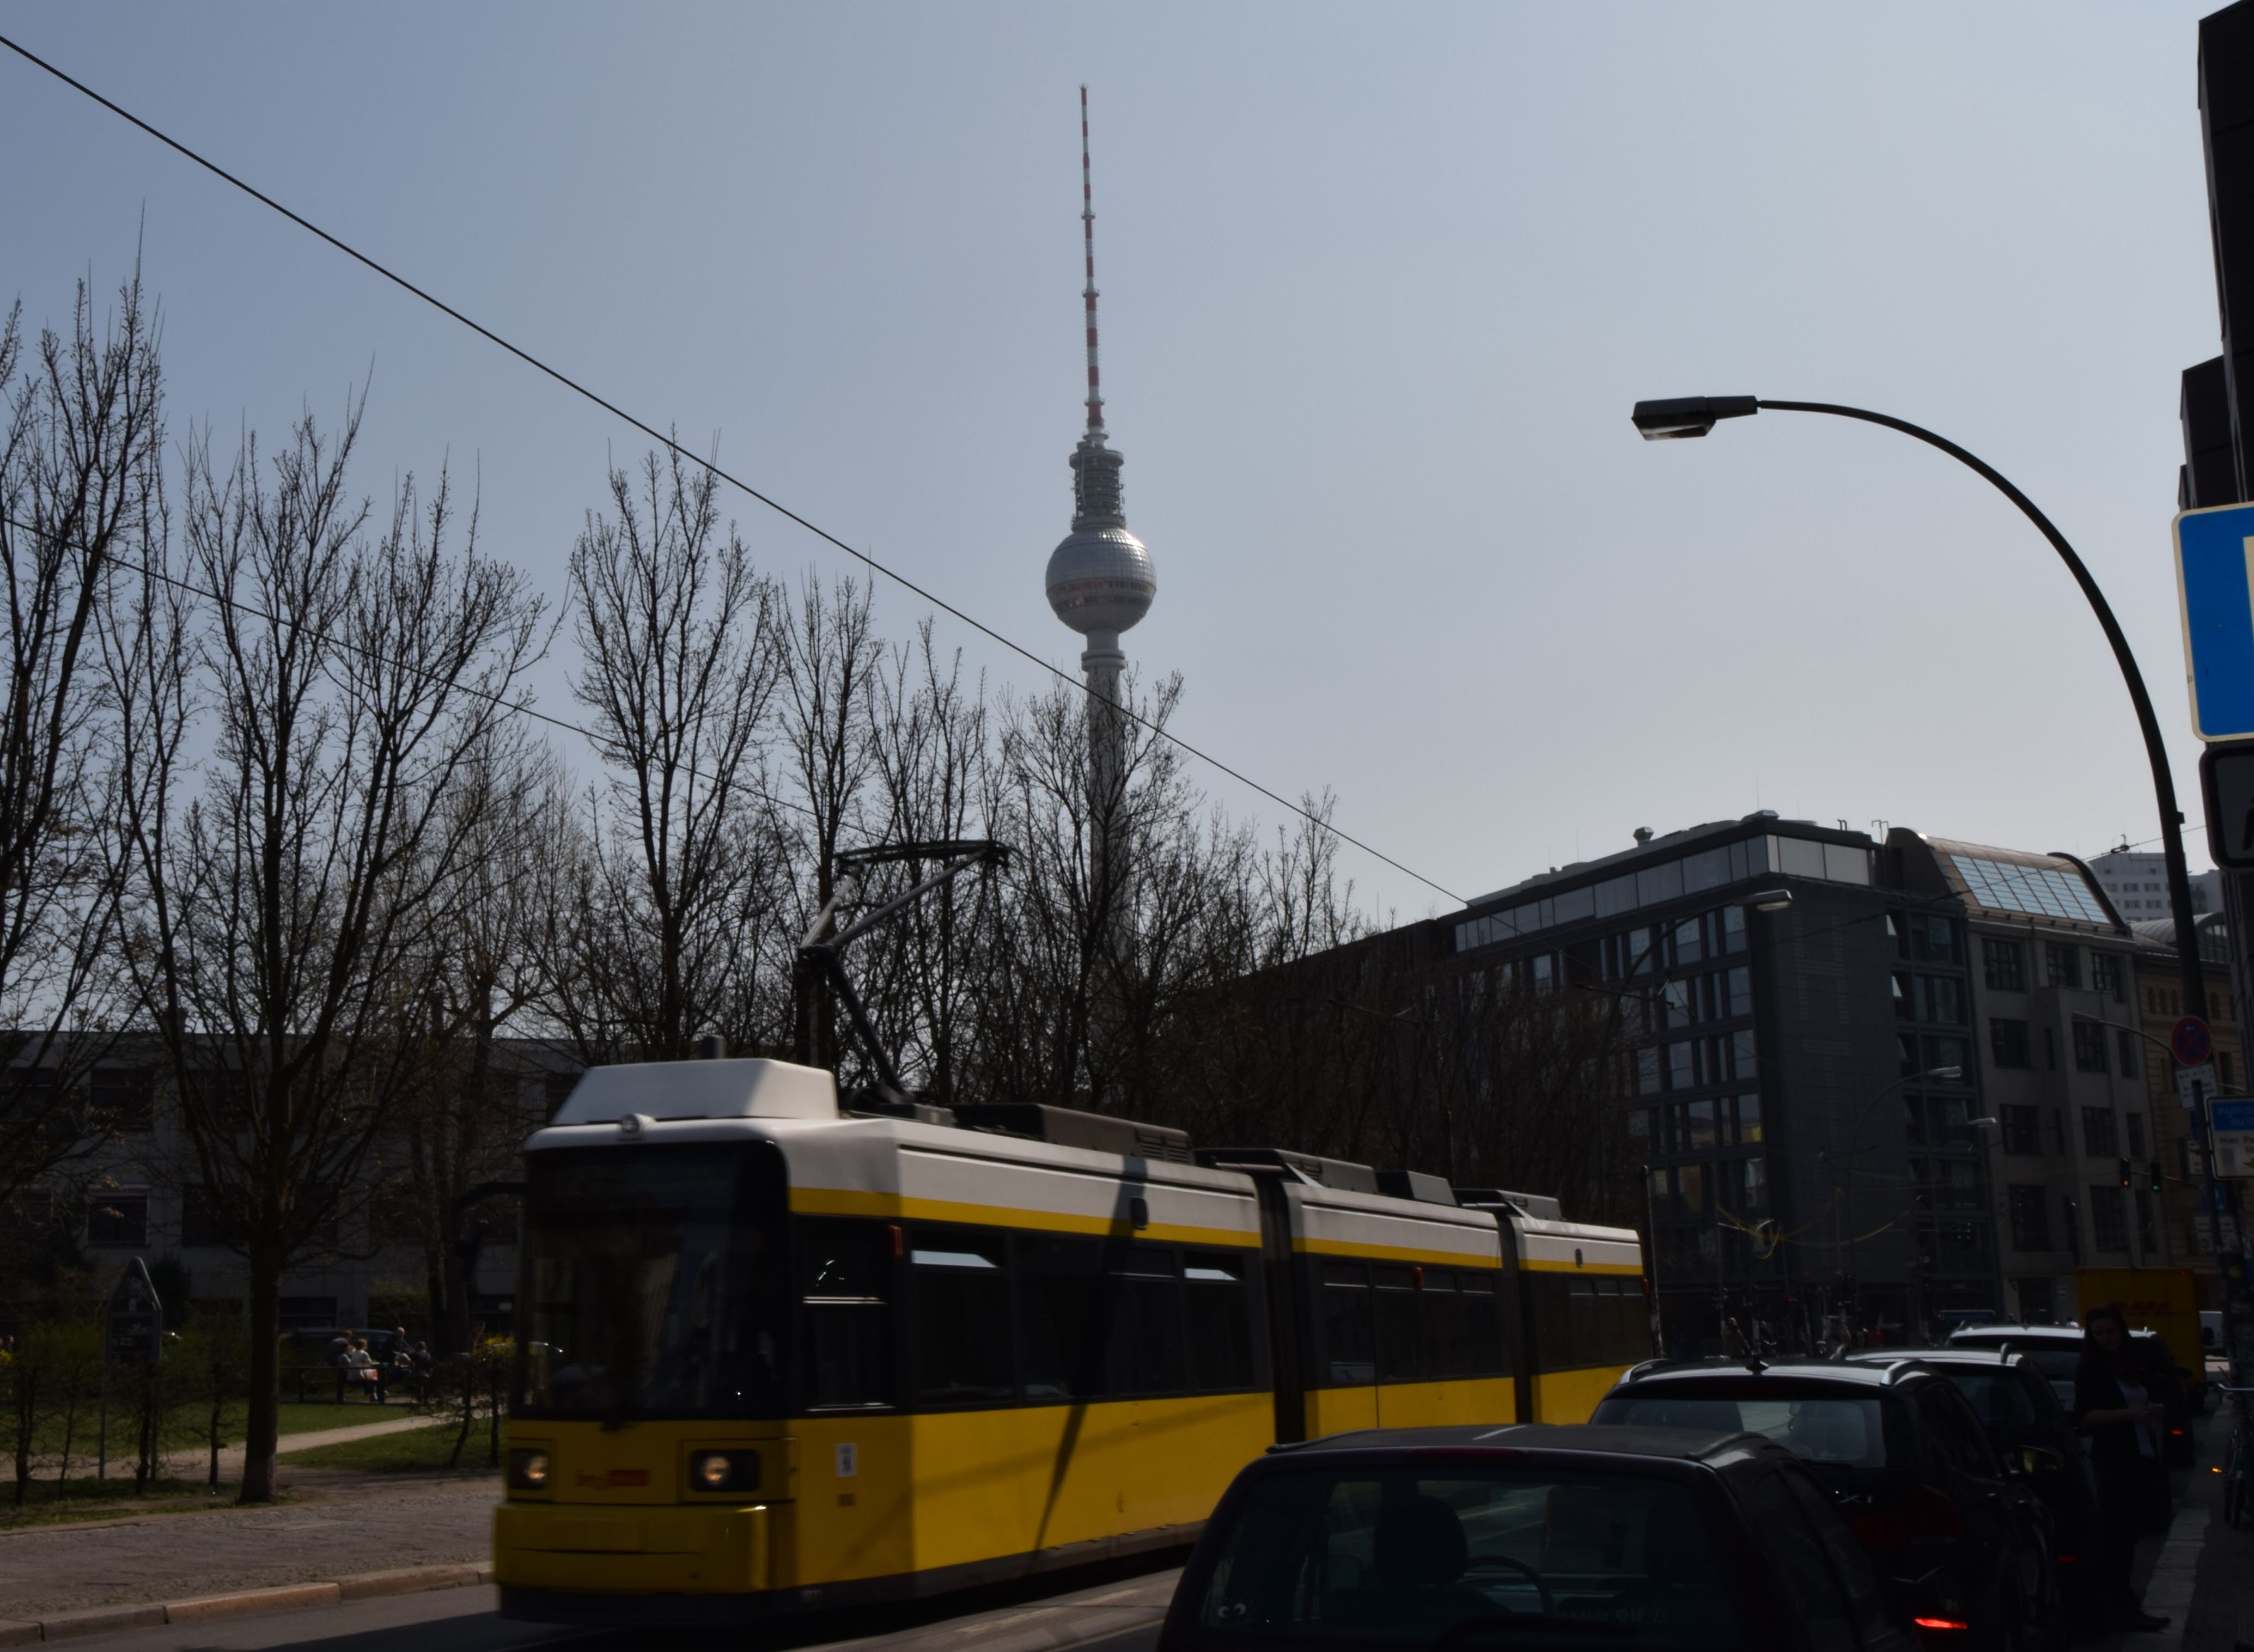
\includegraphics[width=0.99\textwidth]{img/tram}%
	\end{center}
\end{minipage}
\hfill
\begin{minipage}{0.33\textwidth}
	\begin{center}
		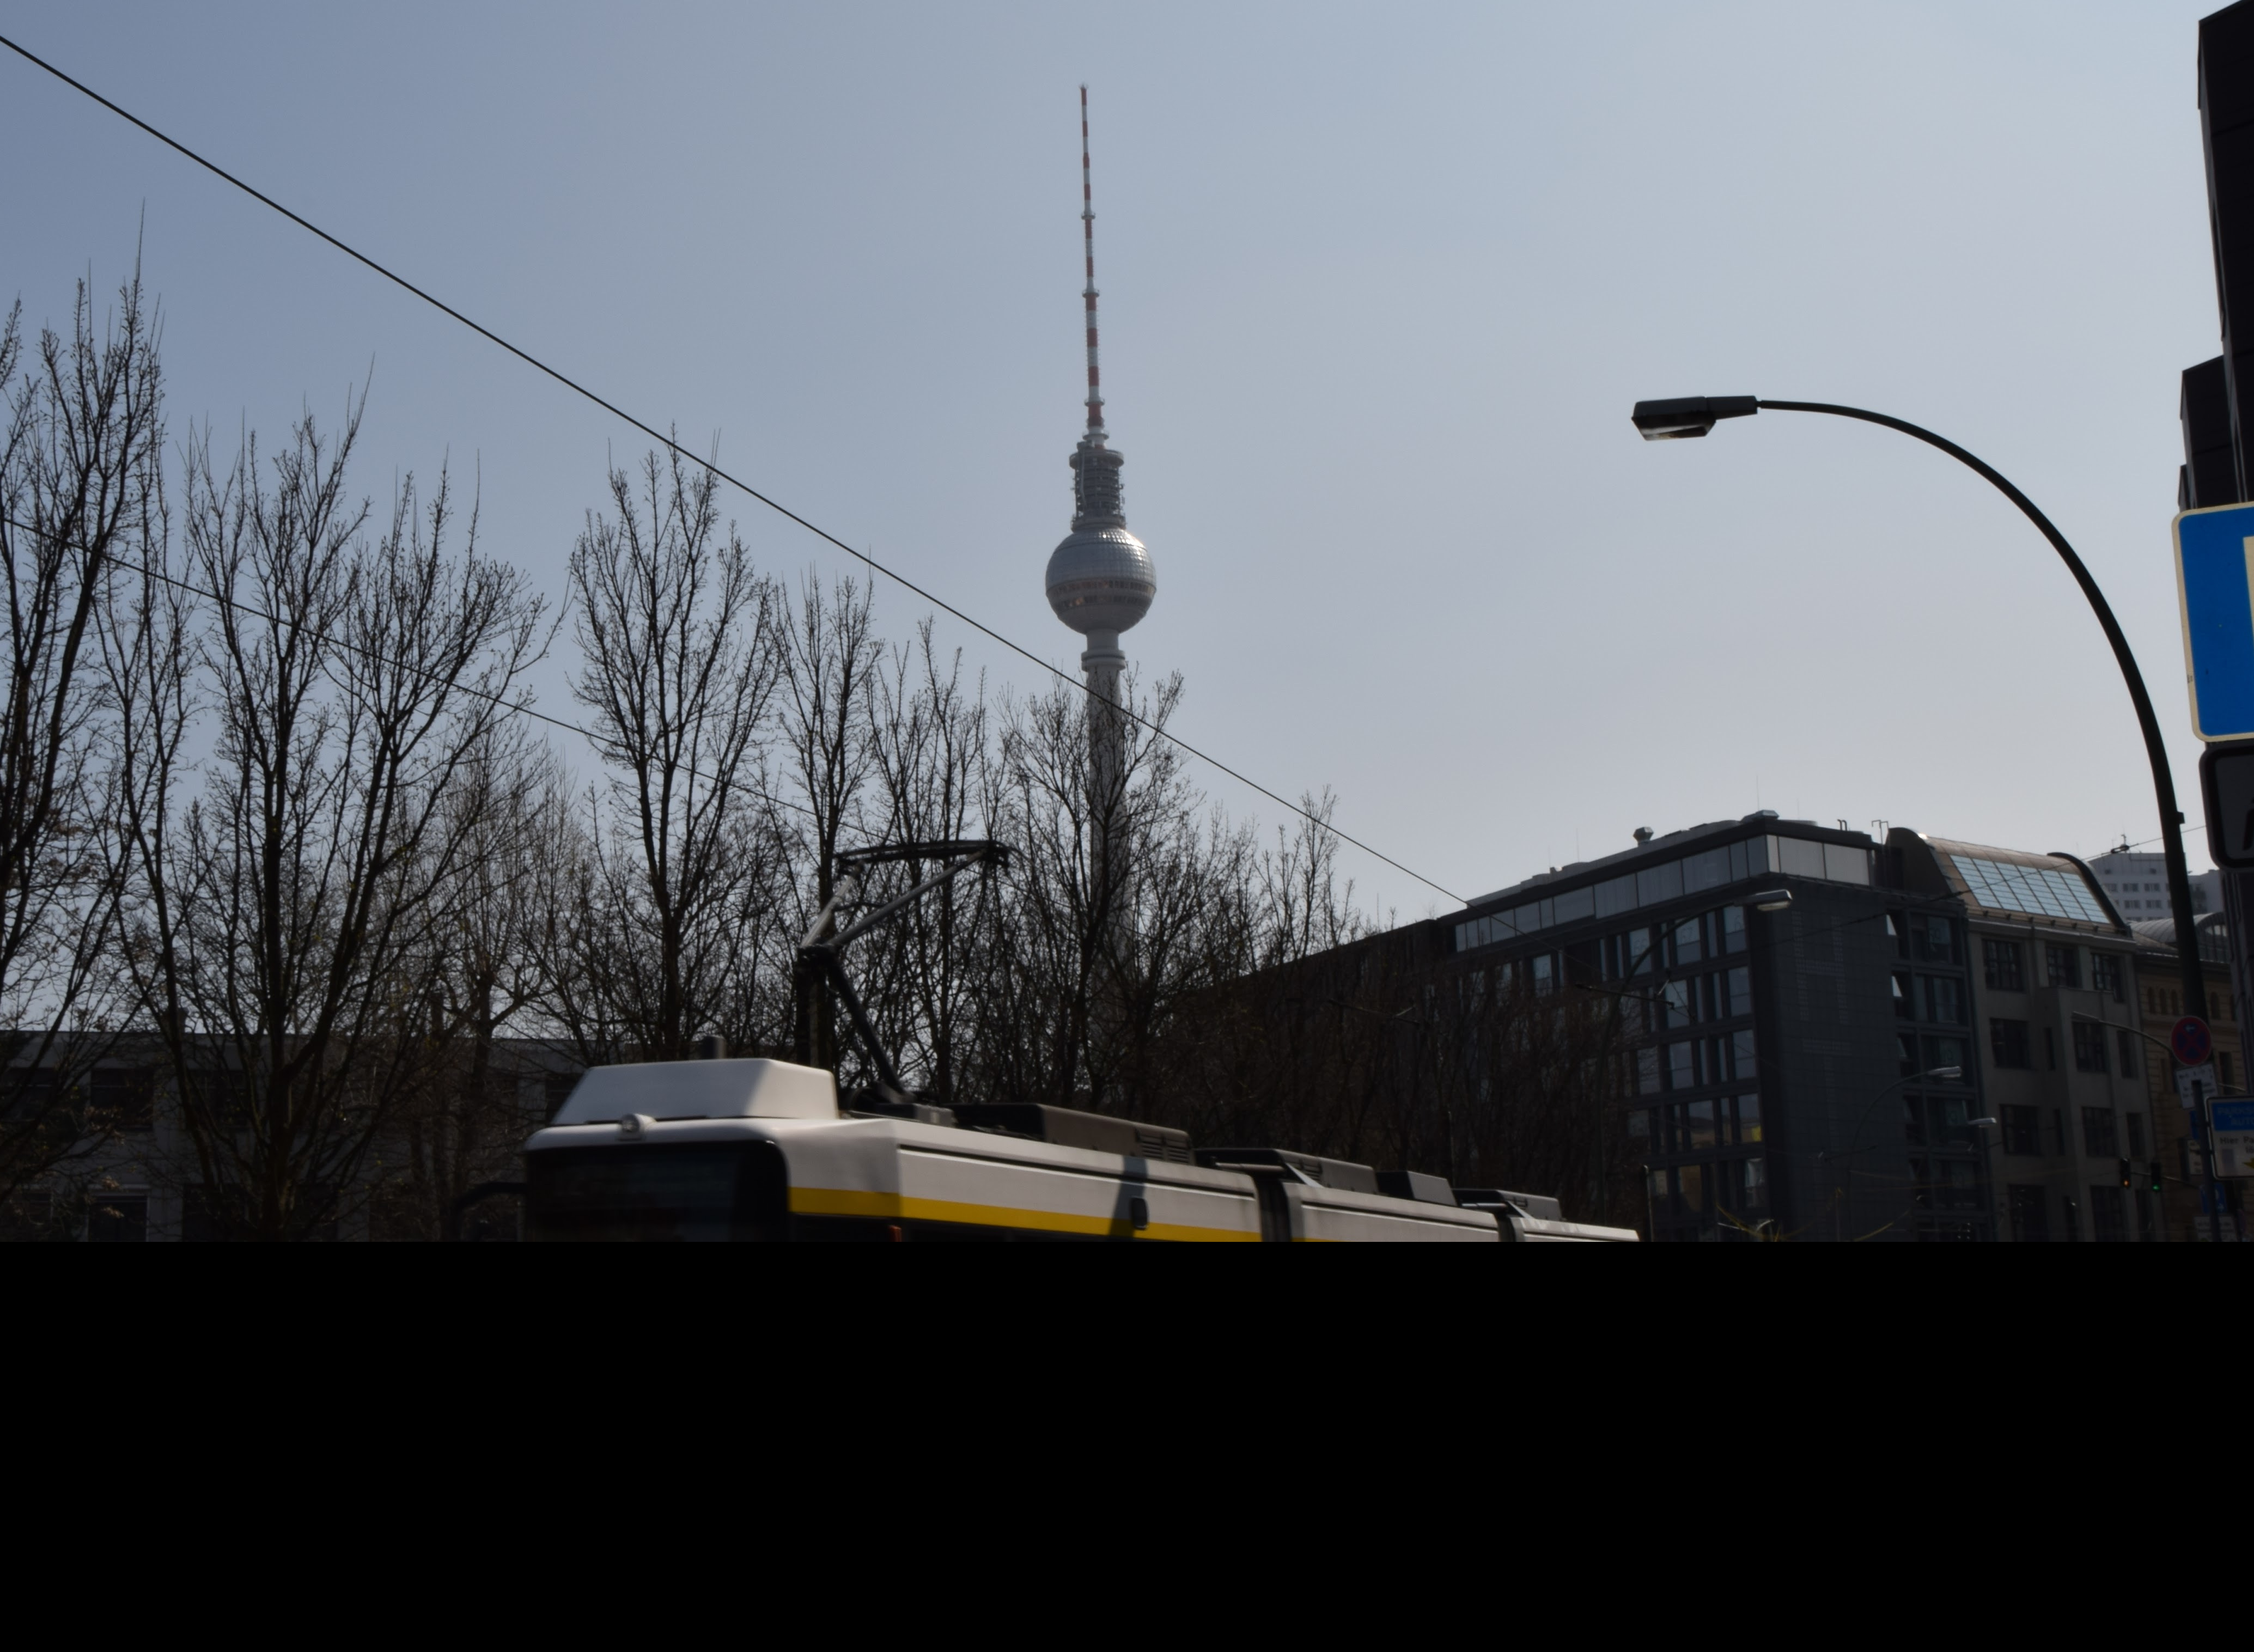
\includegraphics[width=0.99\textwidth]{img/tram_missing}%
	\end{center}
\end{minipage}
\end{minipage}
}



\end{center}

\end{frame}

\subsubsection{Procedure}

\begin{frame}\frametitle{\subsecname:~\subsubsecname}

Let
\slidesonly{\vspace{-5mm}}
\begin{itemize}
\item[]$\vec x \in \R^N$,\\
\item[] w.l.o.g. $\E[\vec x] \eqexcl \vec 0$ (i.e. for each variable $x_i$ its mean $m_i = \sum_{\alpha=1}^{p} x_i^{(\alpha)} \eqexcl 0$)
\end{itemize}

\pause

\begin{enumerate}
\item \underline{Dimensionality Reduction}: From $N$ to $M$: $1 < M\, < N$\\
$\Rightarrow$ simply transmit the first $M$ elements of $\vec x$. 
\pause
\item \underline{Reconstruction}: The recipient reconstructs all $N$ elements by adding zero entries for all missing elements (i.e. \textit{zero-padding}):\\
Let $\widetilde{\vec{x}}$ be the reconstructed observation, where\\ 
 
 \begin{equation}
 % = $ for $j=1,\ldots,M% (perfect reconstruction for the first $M$ elements),
 \widetilde{x}_j = \begin{cases} 
      {x}_j & \text{for}~j=1,\ldots,M \qquad \text{(perfect reconstruction)} \\
      0 & \text{for}~j=M+1,\ldots,N \quad \text{zero-padding} 
   \end{cases}
 \end{equation}
\end{enumerate}

\question{How much error will the recipient accumulate in the case of simple trunction?}

\end{frame}

\subsubsection{Measuring the error}

\begin{frame}\frametitle{\subsecname:~\subsubsecname}

\notesonly{
We measure the MSE between every original point $\vec x$ and its reconstruction $\widetilde{\vec{x}}$.

Let $\widetilde{\vec{x}}$ be the reconstructed observation. }

\slidesonly{\vspace{-7mm}}

\begin{align}
\visible<1->{
\mathit{MSE}  &=  \frac{1}{p} \sum\limits_{\alpha = 1}^p ( \vec{x}^{(\alpha)} - \widetilde{\vec{x}}^{(\alpha)} )^2
	\notesonly{\\&}=  \frac{1}{p} \sum\limits_{\alpha = 1}^p \sum\limits_{j = 1}^M ( {x}_j^{(\alpha)} - \widetilde{{x}}^{(\alpha)}_j )^2\\
	\intertext{The \textcolor{blue}{first $M$} elements were transmitted perfectly, \textcolor{red}{zero padding} is used to extend the vector to its original size of $N$ elements}
}
\visible<2->{
     &=  \frac{1}{p} \sum\limits_{\alpha = 1}^p \bigg(
     \underbrace{
		{\color{blue}\sum\limits_{j = 1}^M} ( x_j^{(\alpha)} - \widetilde{x_j}^{(\alpha)} )^2
		}_{
		\substack{=0 \\\text{ (perfect transmission)}}
		} 
		+ {\color{red}\sum\limits_{j = M+1}^N} ( x_j^{(\alpha)} - 
	\underbrace{
	\vphantom{\sum\limits_{j = 1}^M ( x_j^{(\alpha)} - \widetilde{x_j}^{(\alpha)} )^2}
	\widetilde{x_j}^{(\alpha)}
	}_{\substack{=0\\ \text{padded}}}
	\;)^2 \bigg)\\
     &=  \frac{1}{p} \sum\limits_{\alpha = 1}^p \sum\limits_{j = M+1}^N ( x_j^{(\alpha)} )^2
     \notesonly{\\&}=  \sum\limits_{j = M+1}^N \frac{1}{p} \sum\limits_{\alpha = 1}^p  ( x_j^{(\alpha)} )^2 \\
     &=  \sum\limits_{j = M+1}^N \sigma_j^2
     }
\end{align}

\end{frame}

\begin{frame}

\slidesonly{
\begin{equation}
\mathit{MSE}  =  \frac{1}{p} \sum\limits_{\alpha = 1}^p ( \vec{x}^{(\alpha)} - \widetilde{\vec{x}}^{(\alpha)} )^2 = \sum\limits_{j = M+1}^N \sigma_j^2
\end{equation}
}

In the case of simple trunctation 
the recipient will end up with an MSE equal to $\sum_{j=M+1}^{N} \sigma_j^2$, where $\sigma_j^2$ is the variance of the $x_j$.
\only<1>{
\begin{equation}
\sigma_j^2 = \E\lbrack~(x_j - m_j)^2~\rbrack \stackrel{m_j=0}{=} \E\lbrack~(x_j)^2~\rbrack
\end{equation}
}

\pause

\slidesonly{\vspace{5mm}}

\underline{Objective:} Rotate/Transform the data s.t. truncating the transformed vector $\vec v \in \R^M$ is optimum in the sense of minimal MSE.


\question{Any ideas?}

\pause

- Sort the $N$ component in $\vec x$ from highest to lowest variance. \notesonly{The transformation here would be some permutation of the idenitty matrix that accomplishes the sorting.}\slidesonly{transformation: permutation of identity matrix}

\question{Is this enough?}

- No, we still have to take the \emph{covariances} into consideration.

\end{frame}


\mode*

\clearpage

\mode<all>
\subsection{Variances and Covariances}

\mode<presentation>{
\begin{frame} 
    \begin{center} \huge
        \subsecname
    \end{center}
    \begin{center}And knowing how to read contour plots
    \end{center}
\end{frame}
}

\begin{frame}\frametitle{\subsecname}

Let $\vec x \in \R^N$.

\begin{equation}
\text{Variance}~\sigma_j^2 = \E\Big\lbrack~(x_j - m_j)^2~\Big\rbrack = \frac{1}{p} \sum\limits_{\alpha = 1}^p 
		 \Big( \mathrm{x}_j^{(\alpha)} - m_j \Big)^2 \quad \forall j=1,\ldots,N
\end{equation}

\pause

\begin{equation}
	\text{Covariance matrix } \vec{C} = \big\{ C_{ij} \big\} \quad \text{with} \quad
	C_{ij} = \frac{1}{p} \sum\limits_{\alpha = 1}^p 
		 \Big( \mathrm{x}_i^{(\alpha)} - m_i \Big) 
		 \Big( \mathrm{x}_j^{(\alpha)} - m_j \Big)
\end{equation}

%\vspace{0.7cm}

\begin{equation}
C_{ii} = \sigma^2_i
\end{equation}

$\vec{C}_{N \times N}$ is real and symmetric.

		
\end{frame}

\definecolor{darkgreen}{rgb}{0,0.5,0}
\definecolor{byzantium}{rgb}{0.44, 0.16, 0.39}

\begin{frame}\frametitle{Covariance matrix}

\mode<presentation>{
\only<1>{
\begin{center}
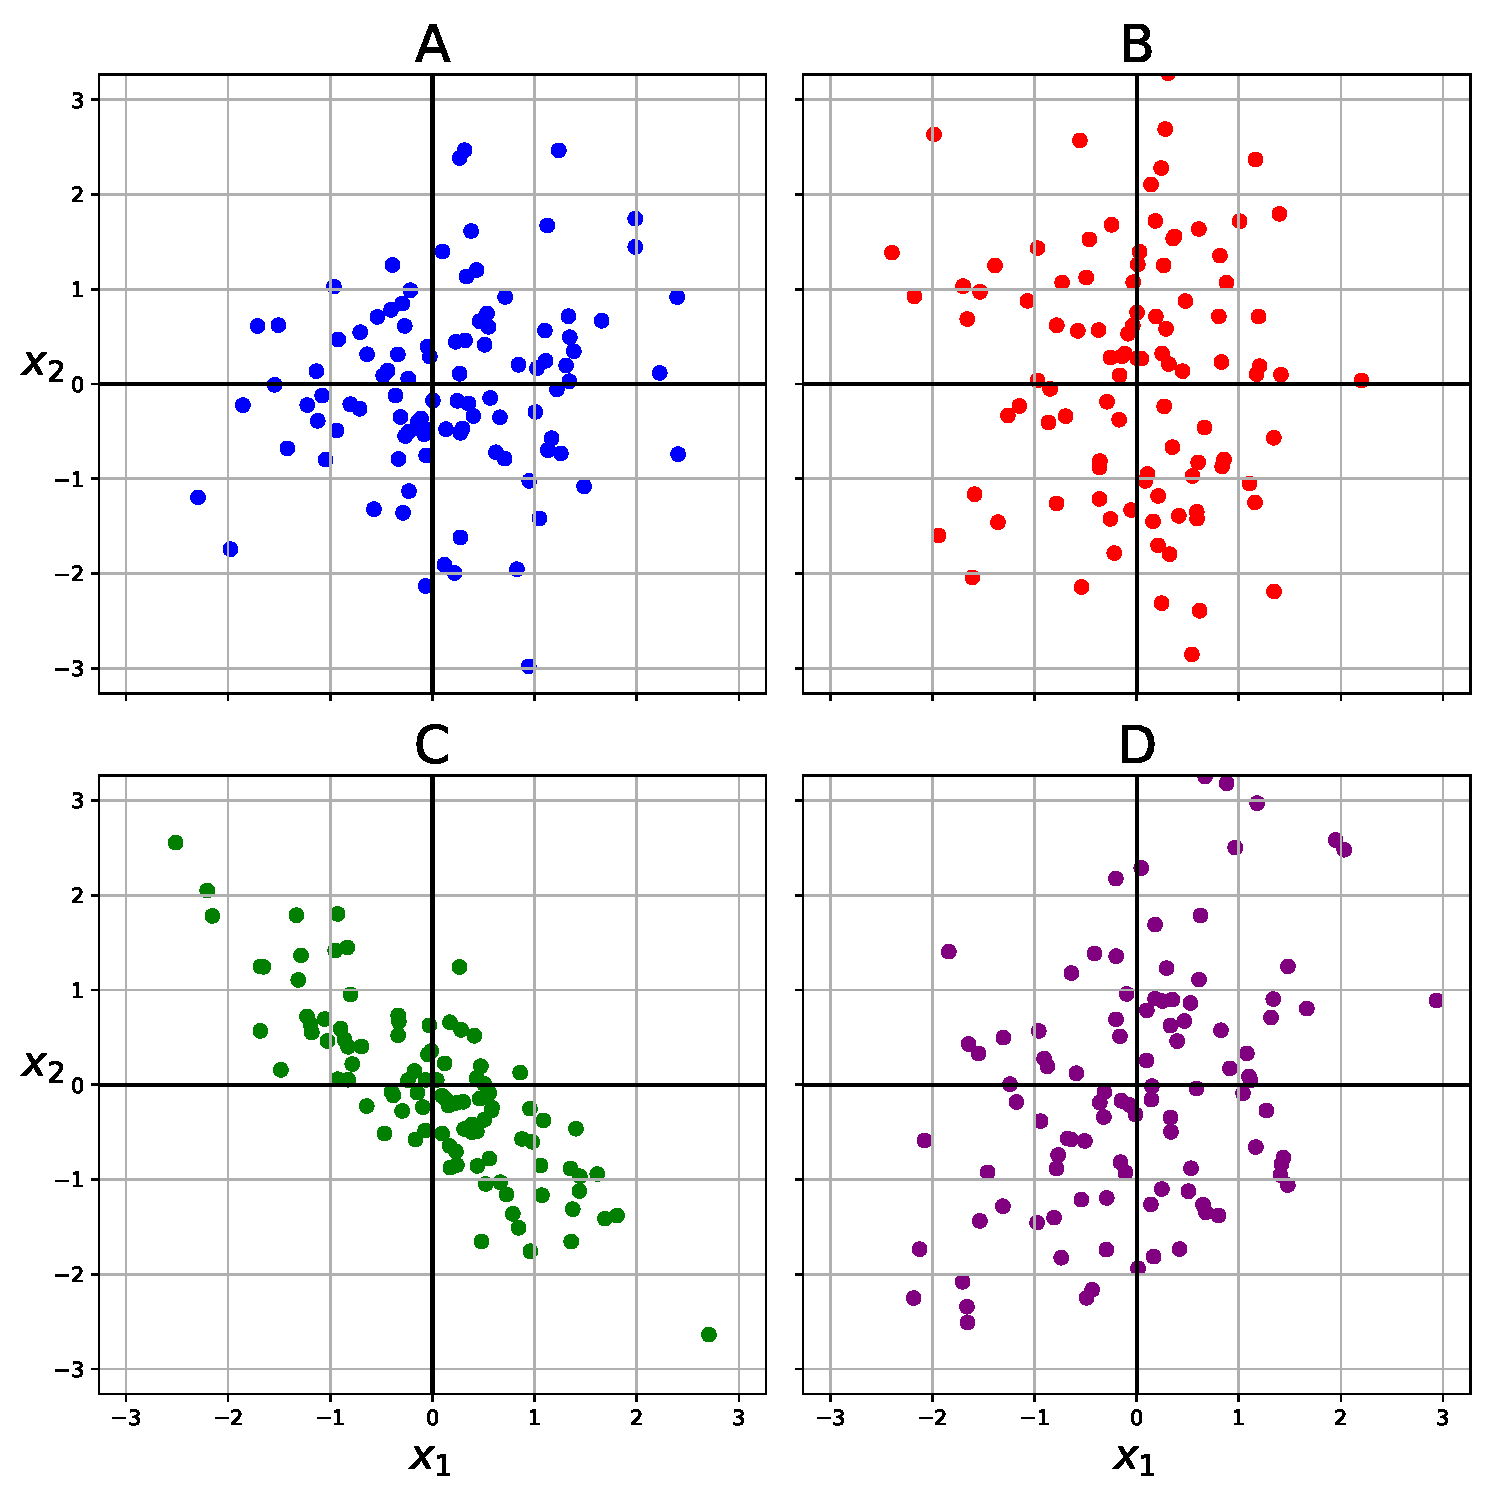
\includegraphics[width=0.6\textwidth]{img/scatter}%
\end{center}
}
\only<2>{
\begin{center}
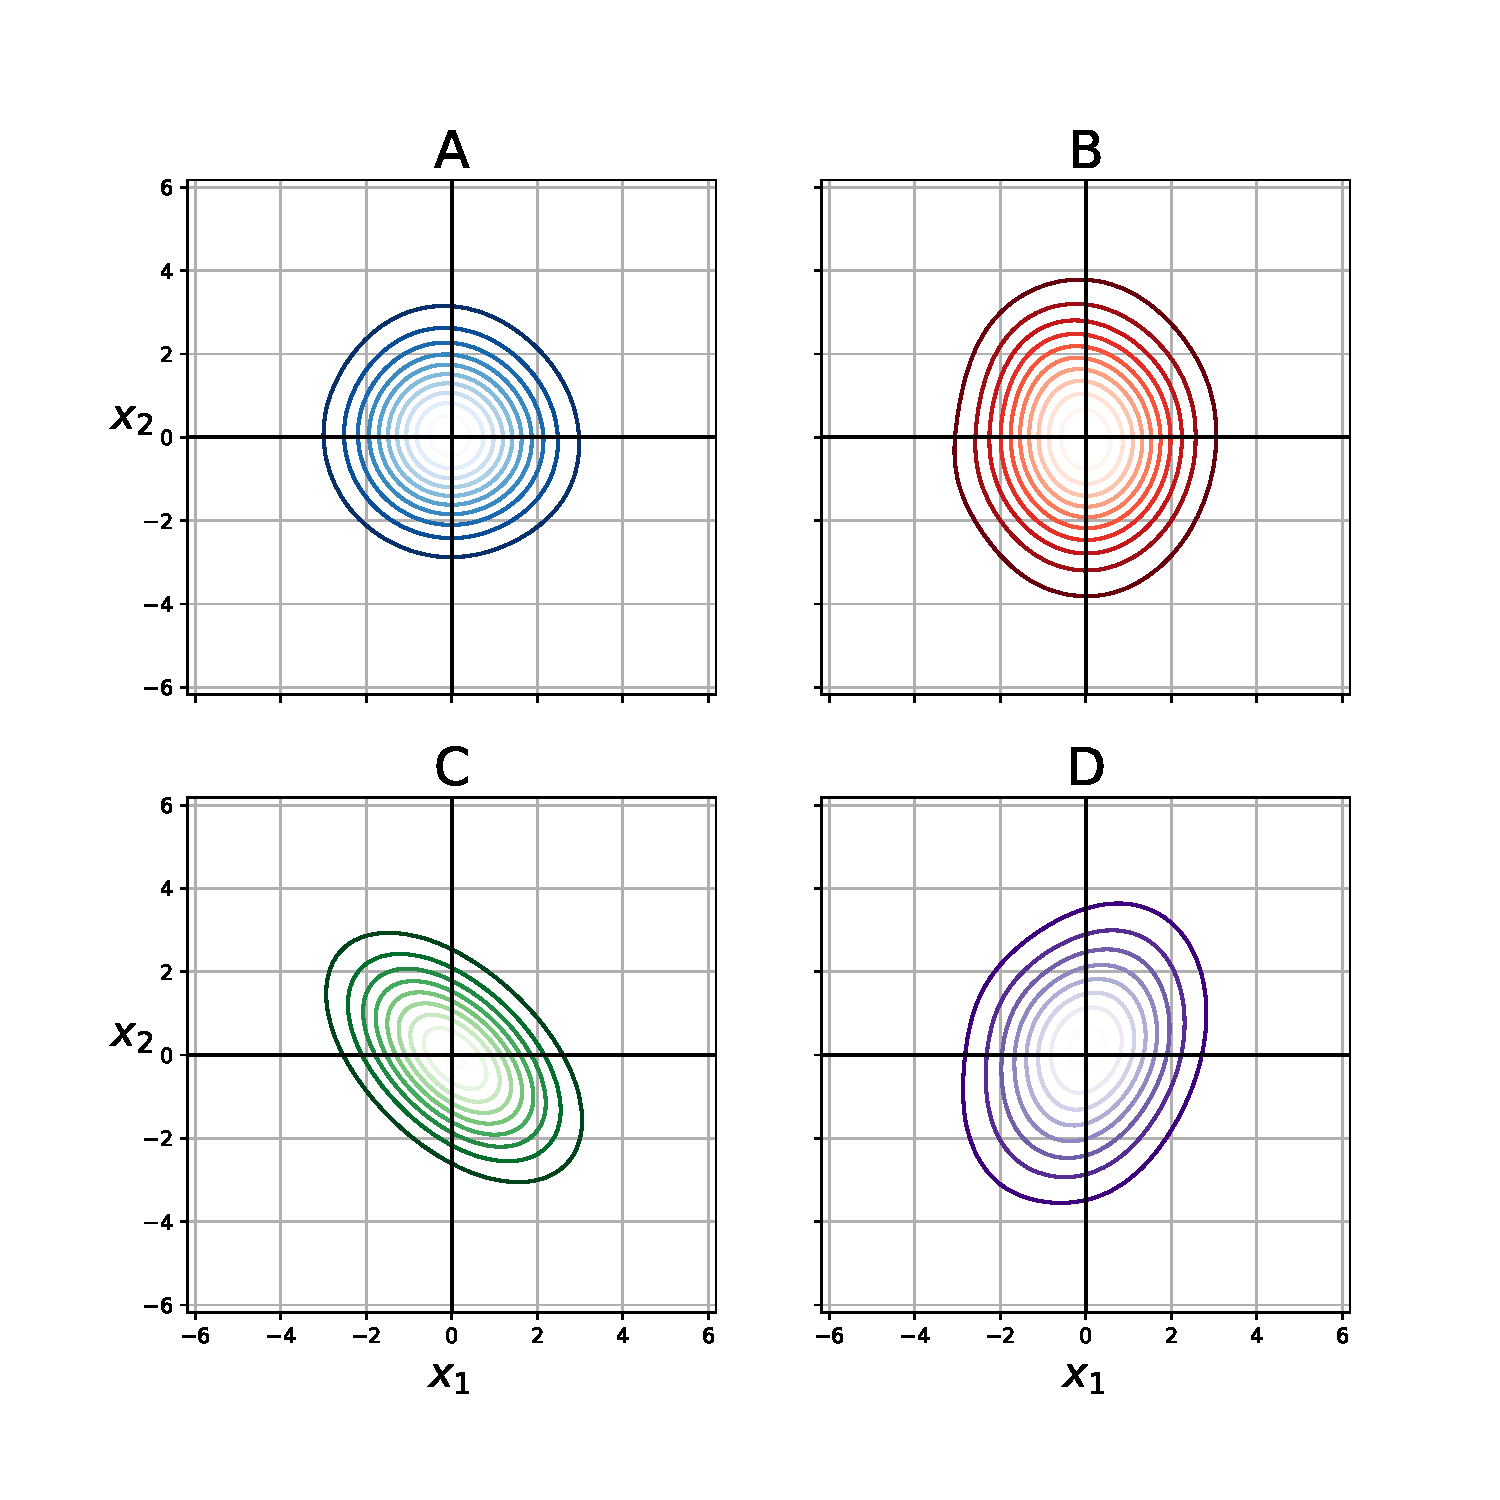
\includegraphics[width=0.6\textwidth]{img/cov}%
\end{center}

\slidesonly{\vspace{-10mm}}
}
}


\mode<article>{

\begin{figure}[ht]
     \centering
     \savebox{\imagebox}{
	 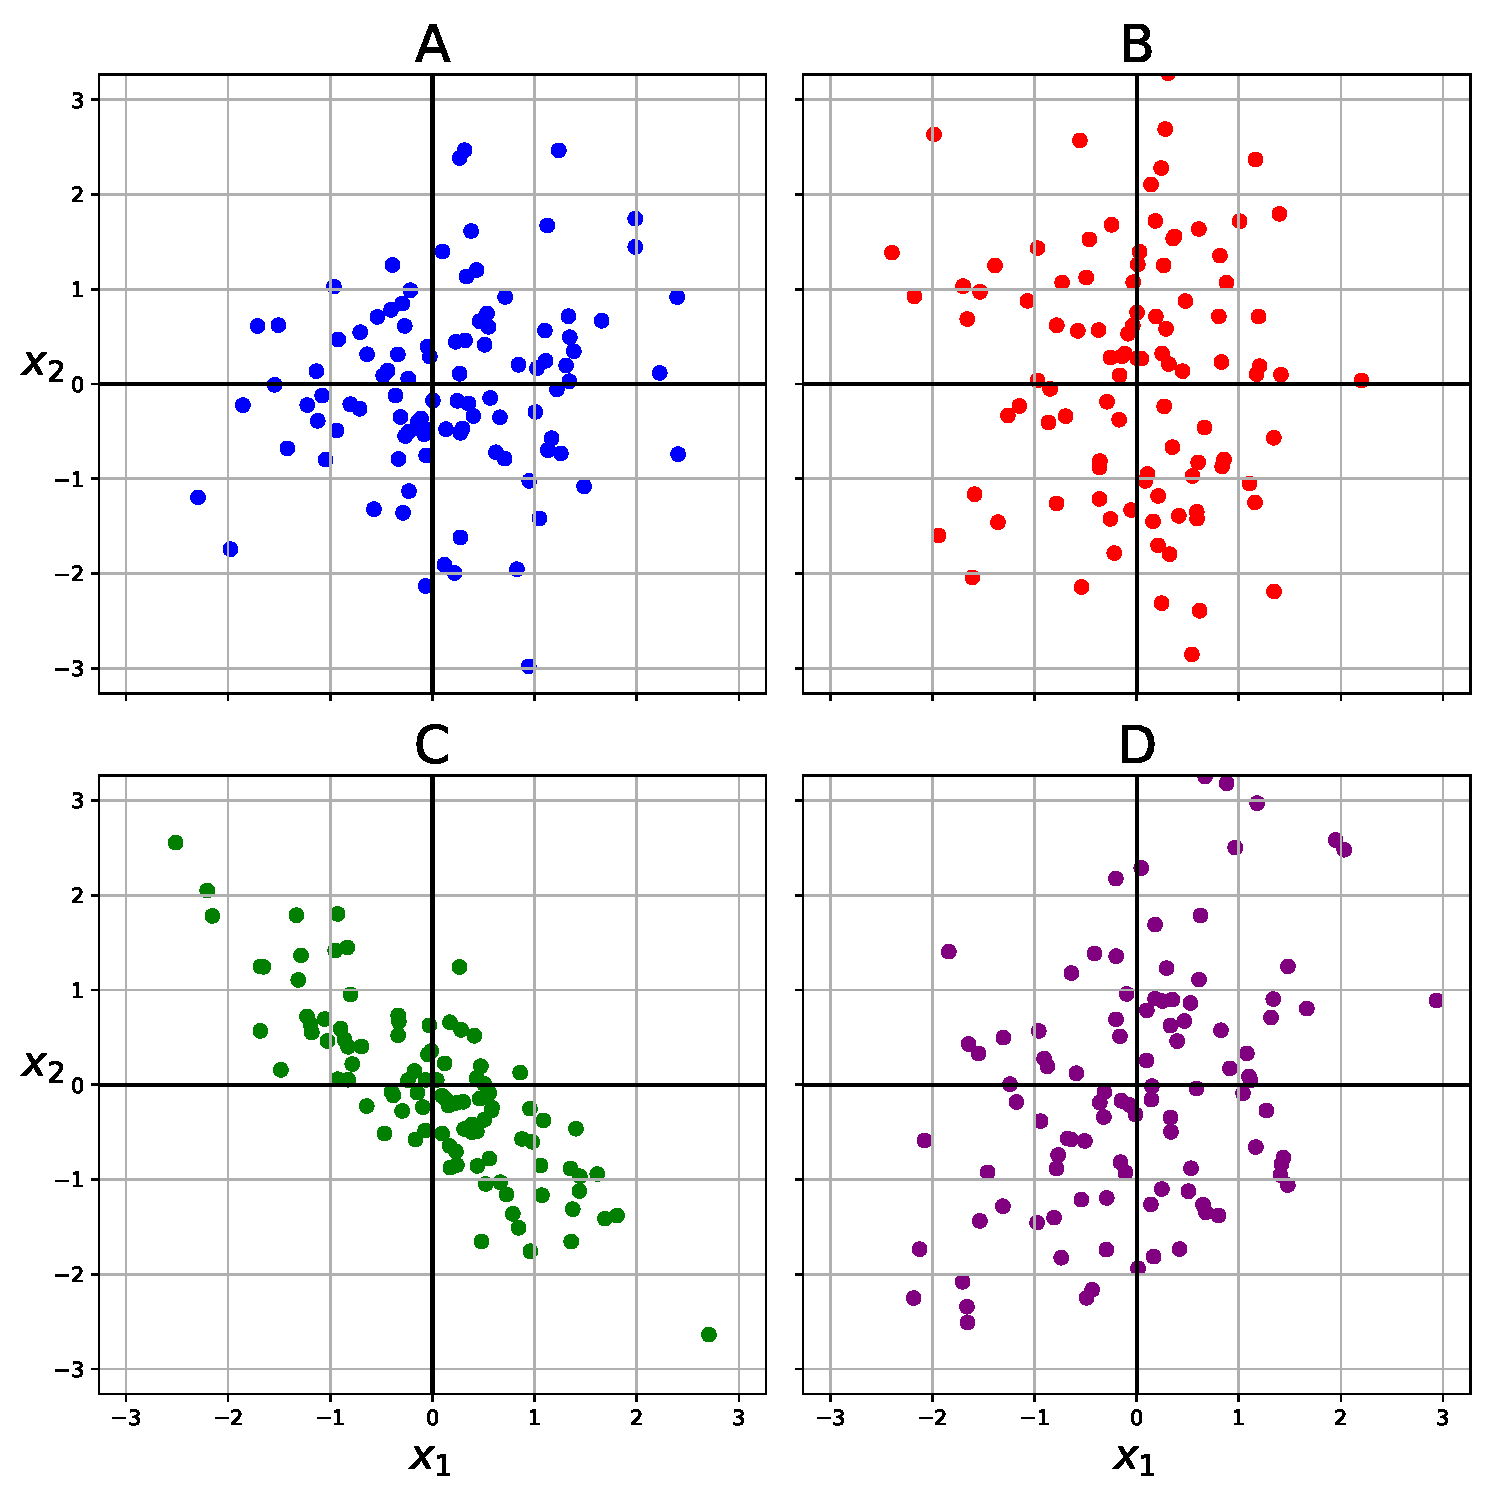
\includegraphics[width=0.28\textwidth]{img/scatter}}%
     \begin{subfigure}[t]{0.28\textwidth}
         \centering
         \usebox{\imagebox}% Place largest image
         \caption{Scatter plots}
     \end{subfigure}
     \hspace{2mm}
     \begin{subfigure}[t]{0.28\textwidth}
         \centering
         \raisebox{\dimexpr.5\ht\imagebox-.5\height}{% Raise smaller image into place
         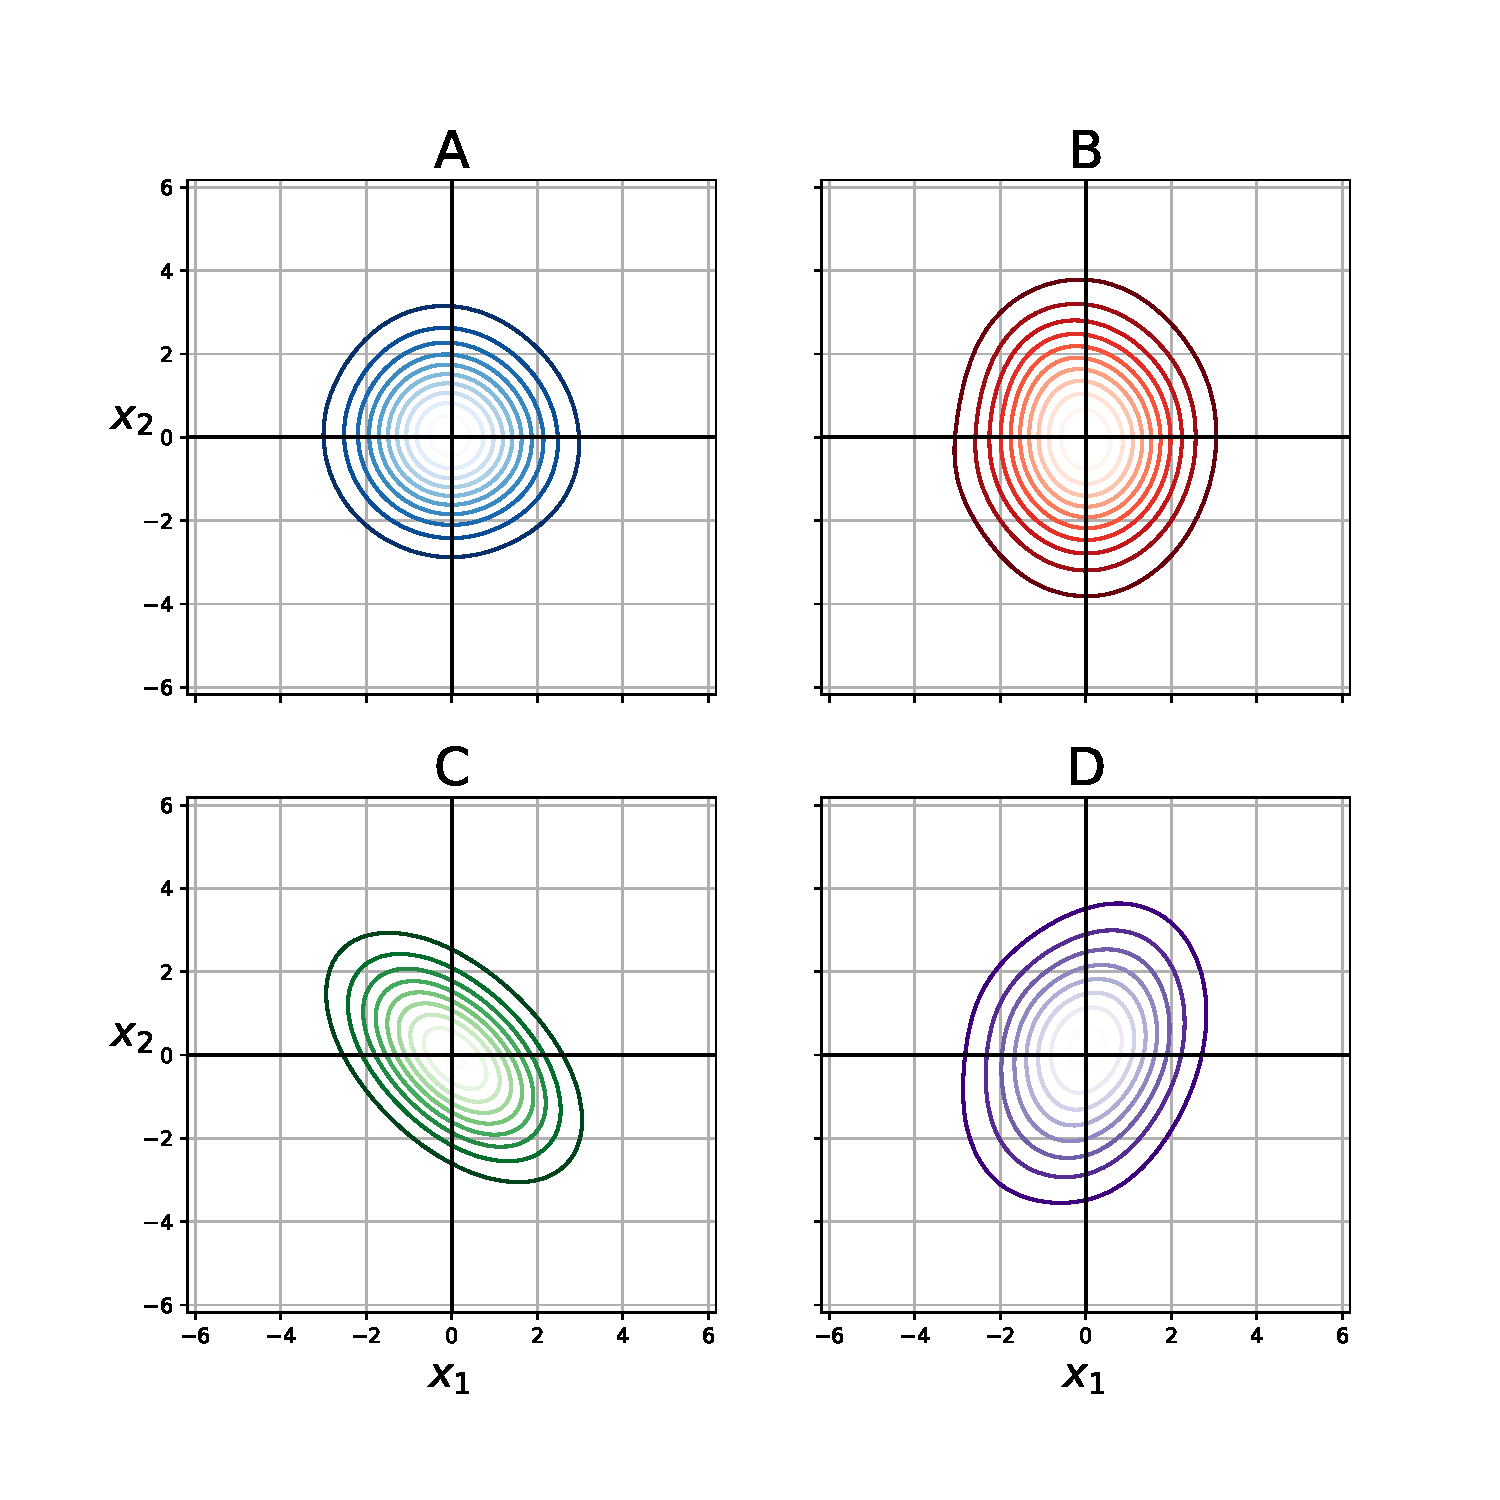
\includegraphics[width=0.99\textwidth]{img/cov}
         }
         \caption{Contour plots}
         \label{fig:linear}
     \end{subfigure}
\end{figure}
}

\question{Define a possible covariance matrix for each of the four datasets above.}

\mode<article>{

\begin{center}
\resizebox{.5\textwidth}{!}{%
\begin{tabular}{rl}
 ${\color{blue}\vec C_\mathrm{A} = \mat{1 & 0 \\ 0 & 1}}$ &  ${\color{red}\vec C_\mathrm{B} = \mat{1 & 0 \\ 0 & 2}}$\\[10mm]
 ${\color{darkgreen}\vec C_\mathrm{C} = \mat{1 & -1 \\ -1 & 1}}$ &  ${\color{byzantium}\vec C_\mathrm{D} = \mat{1 & 0.5 \\ 0.5 & 2}}$
\end{tabular}%
}
\end{center}
}



\end{frame}

\mode*

\clearpage

\mode<all>
\section{PCA}

\mode<presentation>{
\begin{frame} 
    \begin{center} \huge
        \secname
    \end{center}
    \begin{center}
    Transform and rotate the data s.t. keeping only the first $M$ dimensions has minimal MSE.
    \end{center}
\end{frame}
}

\begin{frame}\frametitle{\secname: Procedure}

\begin{enumerate}
	\item Center the data, $\E\lbrack\vec x\rbrack = \vec m  = \frac{1}{p} \sum_{\alpha=1}^{p} \vec x^{(\alpha)}\eqexcl \vec 0$.
	\only<2>{
	\begin{center}
		
\includegraphics[width=5.5cm]{img/meme_center}
    \end{center}
	}
	\visible<3->{
	\item Let $\vec X'$ be the $N \times p$ matrix of the centered data.
	\item Measure the variance of each component in $\vec x_{\mathit{centered}}$. Not enough, the variables in $\vec x$ could be correlated.
	\item Measure covariances $C_{ij}$.
	\item Construct covariance matrix $\vec C$.
		\begin{equation}
		\vec C = \text{Cov}(\vec X') = \mathbf{\Sigma} = \E[\vec X' \vec X'^\top] \in \R^{N \times N}
		\end{equation}
	\item \textbf{eigenvalue decomposition}
	\item Order eigenvalues in descending order. (Highest variance first). The ordered eigenvectors are the \emph{principle components} of the dataset $\vec X$.
	\item Rotate $\vec x_{\mathit{centered}}$ using the first $M$ PCs.
	}
\end{enumerate}


\end{frame}

\subsubsection{Eigenvalue decomposition}

\begin{frame}\frametitle{\subsubsecname}

\begin{equation}
\vec C \, \vec e_a \; = \; \lambda_a \vec e_a  \quad\text{(the eigenvalue problem of PCA)}
\end{equation}

\begin{itemize}
\item[] $\lambda_a: \text{the eigenvalue, the variance along principle component } a.$
\item[] $\vec e_a: \text{the normalized eigenvector, the direction of the } a\text{-th PC in } \R^N$
\end{itemize}

\question{How do we perform an eigenvalue decomposition?}

\pause

\begin{enumerate}
\item Get eigenvalues: $\det(\vec C-\lambda \vec I) = 0$, 
\item Find eigenvector $\vec e_a$ associated with each $\lambda_a$ by solving the linear system\\
$ (\vec C - \lambda_a \vec I )\, \vec e_a = \vec 0$
\footnote{If interested, see {\emph{math\_primer.pdf} on ISIS} for details and an example.}
\end{enumerate}

\end{frame}

\subsubsection{The Scree plot}

\begin{frame}\frametitle{\subsubsecname}

In PCA we sort the eigenvectors from highest to smallest eigenvalue.
Plotting the sorted eigenvalues is referred to as a \emph{scree plot}

\begin{center}
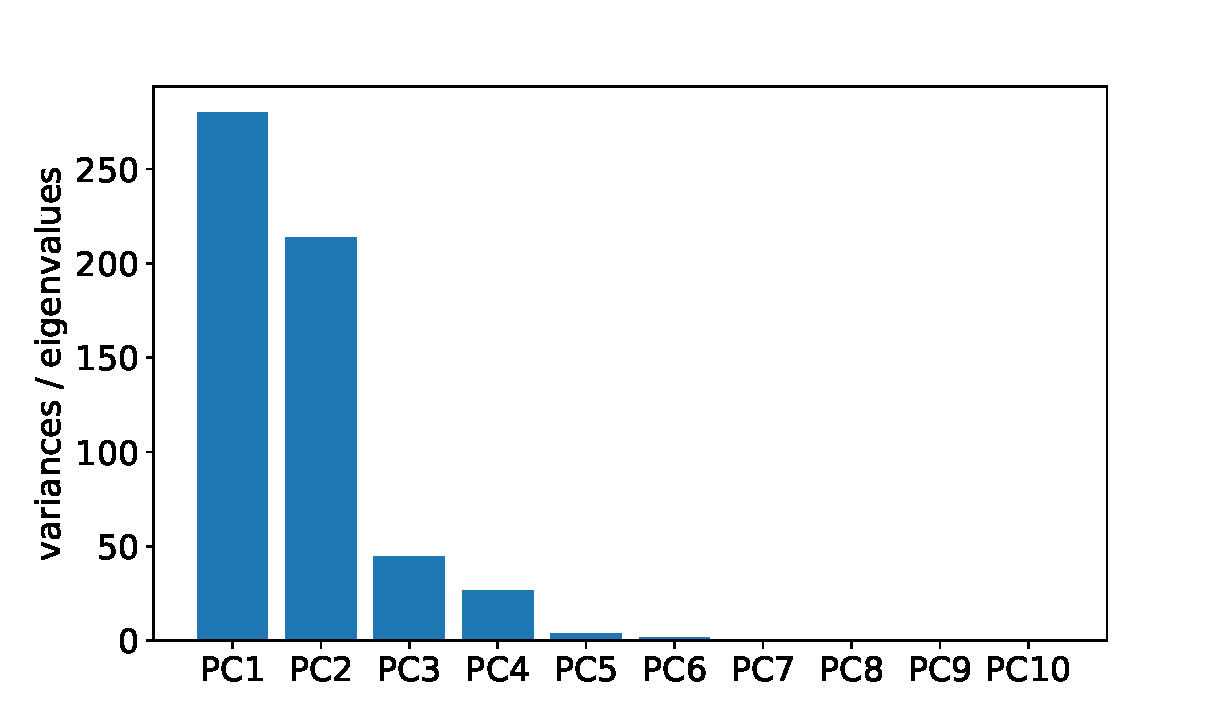
\includegraphics[width=0.6\textwidth]{img/screeplot_kpca_poly_d3}%
\captionof{figure}{Example of a scree plot}
\end{center}

\end{frame}

\subsection{Projection and Reconstruction error}

\begin{frame}\frametitle{How much better is this vs. simple trunctation?}
%\newpage

\only<1,2>{
The transformation onto the PCs is linear:
\begin{equation}
	\vec{x}_{\mathit{centered}} = \underbrace{ a_1 }_{ \vec{e}_1^\top \vec{x} } \vec{e}_1
		+ \underbrace{ a_2 }_{ \vec{e}_2^\top \vec{x} } \vec{e}_2
		+ \ldots
		+ \underbrace{ a_N }_{ \vec{e}_N^\top \vec{x} } \vec{e}_N
\end{equation}

Therefore, we can perfectly reconstruct observations by projecting them from PC space (i.e. feature space) back to the input space. \\
If we only use the \textcolor{red}{first} ${\color{red}M}$ PCs for reconstructing the observations, we will accumulate error.

\svspace{-5mm}

\begin{equation}
\widetilde{\vec{x}} = a_1 \vec{e}_1 + a_2 \vec{e}_2 + \ldots
		+ a_M \vec{e}_M
\end{equation}
}
		
\notesonly{We measure MSE between original centered observations and their corresponding reconstructions just as we did in \eqref{eq:mse}.}

\pause

\only<2,3>{
\begin{equation}
E = \frac{1}{p} \sum_{\alpha = 1}^{p} (\vec x_{\mathit{centered}} - \widetilde{\vec{x}})^2 = \frac{1}{p} \sum_{\alpha = 1}^{p} \sum_{j = M+1}^{N} (a_j^{(\alpha)})^2
\end{equation}
The MSE is equal to the sum of variances of the final $N-(M+1)+1$ components of the \emph{transformed} observations.\\
}
\only<3>{\notesonly{Since the PCs are ordered w.r.t to variance in descending order, }the variances of the last $N-M$ components of the transformed data are smallest.
The transformation is therefore optimal in the sense of minimal MSE.
}

\end{frame}

\mode*

%\clearpage

\mode<all>
\subsection{Applying PCA}

\mode<presentation>{
\begin{frame} 
    \begin{center} \huge
        \subsecname
    \end{center}
    \begin{center}What can we do with PCA?
    \end{center}
\end{frame}
}


\begin{frame}\frametitle{\subsecname}

\begin{enumerate}
\item Dimensionality reduction
\item Visualization (e.g. plot the projections onto the first 2 or 3 PCs.)
\item Whitening (i.e. decorrelate the data) - exploit that eigenvectors form an orthonormal basis.
$$
\vec v^{(\alpha)} = \vec x_{whitened}^{(\alpha)} = \vec{\Lambda}^{-\frac{1}{2}}\vec{M}^\top\vec{x}^{(\alpha)}
\quad
\forall \alpha
$$

\question{What is the covariance of $\vec x_{whitened}$?}

\pause

-the Identity matrix.

\end{enumerate}

\end{frame}

\newpage


\subsubsection{A note on implementation:}

\begin{frame}\frametitle{\subsubsecname}

\question{Is an off-the-shelf implementation such as\\ sklearn.decomposition.PCA for python really necessary?}

PCA boils down to solving the eigenvalue problem.
We bascially need a routine with which to solve the eigenvalue problem. For python, the obvious choice is to use a routine like \textit{numpy.linalg.eig(A)}. \emph{Whatch out for how to intepret the output.}

\end{frame}

\begin{frame}{Only}\frametitle{\subsubsecname}

\svspace{-5mm}

\question{Are there alternatives to eigenvalue decomposition?}

\notesonly{Yes, namely,}

\underline{Singular Value Decomposition (SVD)}:\\
Let $\vec X' \in \R^{N \times p}$ be the centered dataset (centering is a must):
\begin{equation}
\vec X'_{N \times p} = \vec U_{N \times N} \, \vec S_{N \times p} \, \vec V^\top_{{p \times p}}
\end{equation}
\svspace{-5mm}
where,
\begin{equation}
\vec U^\top \vec U = \vec I_{N \times N}
\notesonly{
\end{equation} and 
\begin{equation}
}
\slidesonly{\quad \text{and} \quad}
\vec V^\top \vec V = \vec I_{p \times p}
\end{equation} (i.e. $\vec U$, $\vec V$ are orthogonal).
\begin{itemize}

\item<only@2> The columns of $\vec V$ (or rows of $\vec V^\top$) make up the eigenvectors of $\vec X'^\top\vec X'$.
\item<only@3,4,5> The columns of $\vec U$ make up the eigenvectors of $\vec X'\vec X'^\top$.
\item<only@4,5> $\vec S$ is a diagonal matrix. The singular values in $\vec S$ (the diagonal entries) are the \textbf{square roots} of the  eigenvalues of the eigenvectors of $\vec X'\vec X'^\top$ or $\vec X'^\top\vec X'$.
\end{itemize}

\only<5>{
Recall:
$$
\vec C = \E[\vec X' \vec X'^\top] = \frac{1}{p} \vec X' \vec X'^\top
$$
}

\end{frame}

\begin{frame}\frametitle{\subsubsecname}

\question{When to use SVD vs. Eig? \textbf{Not dogma}}

\begin{itemize}

\item Numerical instabilities in eigendecomposition of very large covariance matrix $\rightarrow$ SVD
\item SVD not applicable to Kernel-PCA $\rightarrow$ Eig
\item Computational efficiency $\rightarrow$ SVD (depends...?)
\end{itemize}

\slidesonly{
$$
\vec X' \in \R^{N \times p} \quad \leadsto \quad \vec C = \frac{1}{p} \vec X' \vec X'^\top
$$
}

\end{frame}

\mode*

\clearpage

%\section{References}
%\begin{frame}[allowframebreaks] \frametitle{References}
	%\scriptsize
	%\bibliographystyle{plainnat}
	%\bibliography{bibliography}
%\end{frame}

\end{rightcolumn}
\end{paracol}

\end{document}
